\documentclass[bachelor, och, labwork]{shiza}

\usepackage[utf8]{inputenc}
\usepackage{graphicx}

\usepackage[sort,compress]{cite}
\usepackage{amsmath}
\usepackage{amssymb}
\usepackage{amsthm}
\usepackage{fancyvrb}
\usepackage{longtable}
\usepackage{array}
\usepackage[english,russian]{babel}
\usepackage{minted}

\usepackage{tempora}


% \usepackage[colorlinks=false]{hyperref}


\newcommand{\eqdef}{\stackrel {\rm def}{=}}


\begin{document}

\title{Алгоритмы алгебры и теории чисел}

\course{4}

\group{431}

\napravlenie{10.05.01 "--- Компьютерная безопасность}


\author{Никитина Арсения Владимировича}


\satitle{доцент}
\saname{А.\,С.\,Гераськин}


\date{2022}

\maketitle

% Включение нумерации рисунков, формул и таблиц по разделам
% (по умолчанию - нумерация сквозная)
% (допускается оба вида нумерации)
%\secNumbering


\tableofcontents

\section{Задание лабораторной работы}

Осуществить построение большого простого числа с использованием теоремы 
Поклингтона.

\section{Теоретическая часть}

\begin{center}
    \textit {Теорема Поклингтона}
\end{center}

Пусть $n=q^{k}R+1$ где $q$ --- простое число, $k\geqslant 1$. Если существует 
такое целое число $a$, что $a^{n-1} \equiv 1 \pmod n$ и НОД$(a^{{(n-1)}/q}-1,n)=1$, 
то каждый простой делитель $p$ числа $n$ имеет вид $p=q^{k}r+1$ при некотором 
натуральном $r$.

\begin{center}
    \textit {Доказательство}
\end{center}

Пусть $p$ --- простой делитель числа $n$. Тогда из условия теоремы вытекает, 
что $a^{n-1}=1{\pmod {p}}$ и $a^{(n-1)/q}\neq 1{\pmod {p}}$. Отсюда получаем, 
что порядок $m$ элемента $a$ по модулю $p$ удовлетворяет условиям: $n-1=md$, где
$d$ --- некоторое целое. Допустим, $q$ делит $d$. В этом случае $(n-1)/q=m(d/q)$,
где $(d/q)$ --- целое. Следовательно $a^{(n-1)/q}=1{\pmod {p}}$, что невозможно. 
Поскольку $n-1=md=q^{k}R$, то $m$ делится на $q^k$. Однако $m$ должно делить 
число $p-1$. Следовательно, $p=q^{k}r+1$ при некотором $r$. Теорема доказана.

\begin{center}
    \textit {Критерий Поклингтона}
\end{center}

Пусть $n$ --- натуральное число. Пусть число $n-1$ имеет простой делитель $q$, 
причем $q>{\sqrt {n}}-1$. Если найдётся такое целое число $a$, что выполняются 
следующие два условия:

\begin{enumerate}
    \item $a^{n-1} \equiv 1 \pmod n$,
    \item числа $n$ и $a^{(n-1)/q}-1$ взаимнопросты,
\end{enumerate}

то $n$ --- простое число.

\begin{center}
    \textit {Доказательство}
\end{center}

Предположим, что $n$ является составным числом. Тогда существует простое число
$p$ --- делитель $n$, причем $p<{\sqrt {n}}$. Заметим, что $q>p-1$, следовательно
$q$ и $p-1$ --- взаимнопросты. Следовательно, существует некоторое целое число 
$u$, такое, что $uq\equiv 1{\pmod {p-1}}$. Но в таком случае 
$a^{(n-1)/q}\equiv a^{uq(n-1)/q}=a^{u(n-1)}\equiv 1{\pmod {p}}$ (в силу условия 1). 
Но таким образом получено противоречие условию 2. Следовательно, $n$ является 
простым числом.



\section{Практическая часть}
\subsection{Пример работы алгоритма}
\begin{figure}[H]
    \centering
    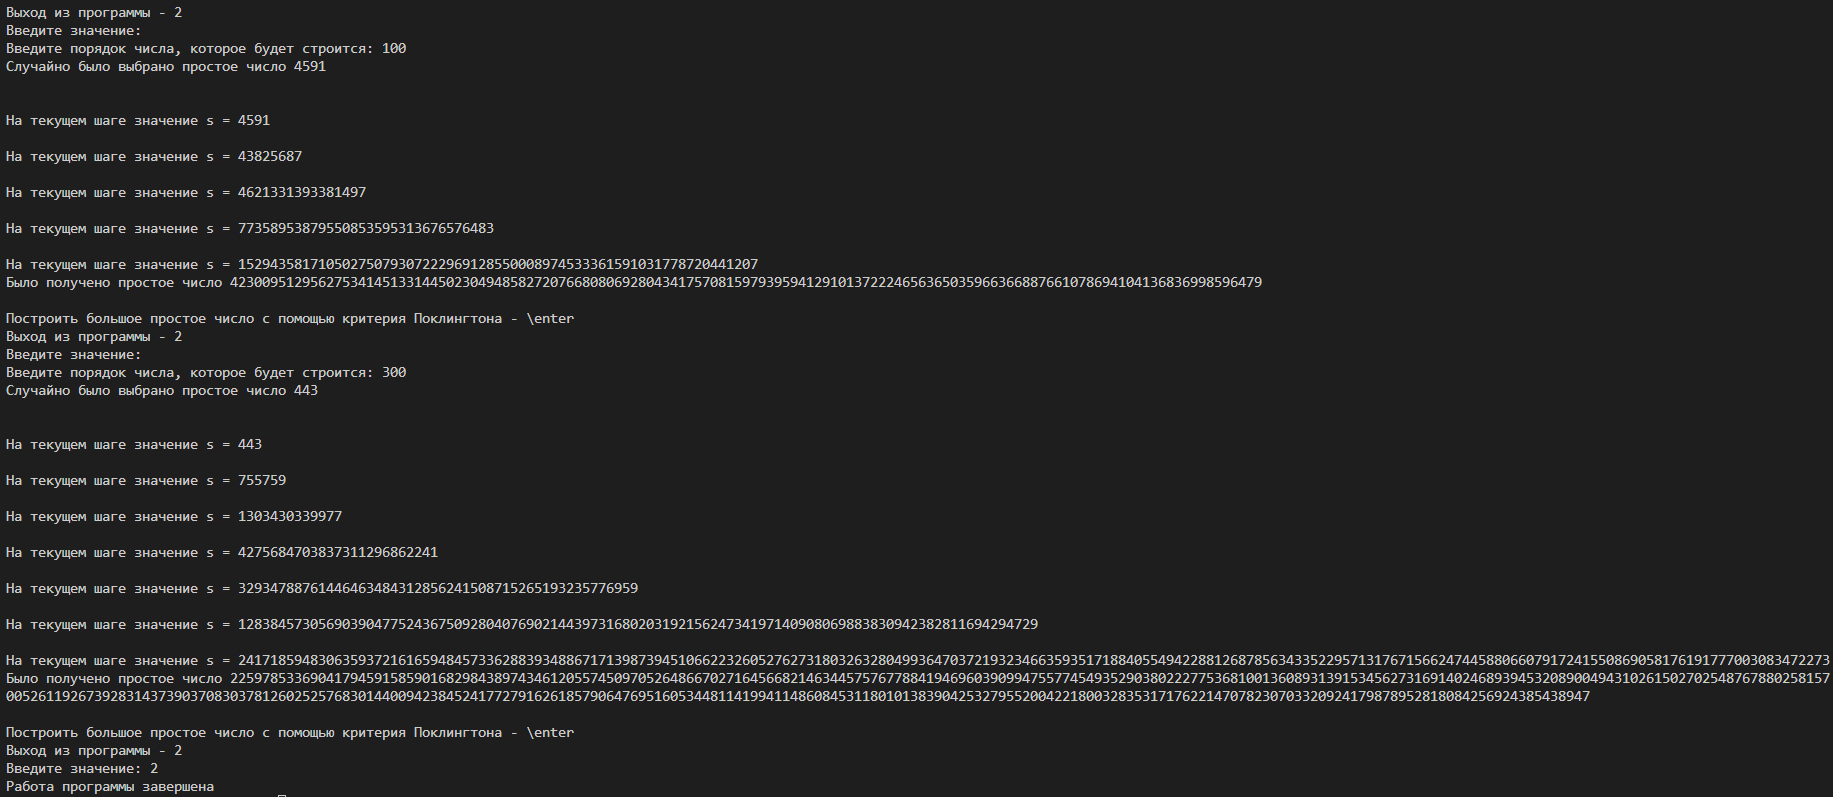
\includegraphics[width=1\textwidth]{pic1.png}
    \caption{}
\end{figure}

\setminted[python]{linenos,breaklines=true, fontsize=\small, style=bw}
    \subsection{Код программы, реализующей рассмотренный алгоритм}
        \inputminted{python}{lab10.py}

\end{document}